\label{sec:Servidor}

\section{Estructura}
	S'utilitzarà una Raspberry Pi 2 com a servidor de proves. La idea és que l'usuari pugui accedir a una aplicació web per utilitzar el sistema, ja sigui desde Internet o des d'una xarxa local.\\\\
	L'estructura d'aquest servidor serà la següent:\\
	\begin{figure}[H]
			\centering
			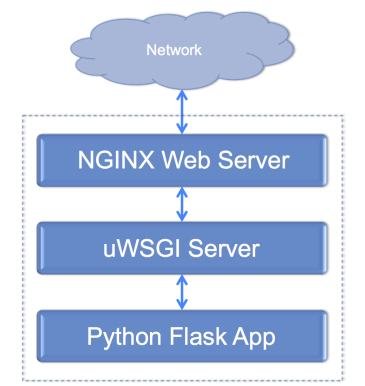
\includegraphics[width=0.6\textwidth]{images/server}
			\caption[Estructura del servidor]{Estructura del servidor\protect\footnotemark}
	\end{figure}
	\footnotetext{\textbf{Font:} https://iotbytes.wordpress.com}
	\subsection{Flask}
		Per desenvolupar l'aplicació web he decidit utilitzar Flask\cite{Flask}, un micro-framework de Python que permetrà utilitzar el codi desenvolupat del projecte amb facilitat.
		A més, també permet utilitzar un servidor per provar l'aplicació en la fase de desenvolupament sense necessitat d'inicialitzar el servidor web.\\\\
		Un exemple d'aplicació en Flask (el típic Hello World) seria així:\\
		\begin{python}
from flask import Flask
app = Flask(__name__)

@app.route("/")
def hello():
	return "Hello World!"

if __name__ == "__main__":
	app.run()
		\end{python}
	\subsection{Nginx}
		Nginx\cite{Nginx} és un servidor web i proxy invers lleuger i d'alt rendiment. Com que s'ha decidit utilitzar una Raspberry com a servidor de proves, Nginx és una bona opció, ja que no consumeix gaires recursos
		i ofereix molt bon rendiment.\\\\
		Nginx, però, no és capaç de comunicar-se amb l'aplicació web per WSGI. Per tant, necessitarem instal·lar un altre servidor que faci d'intermediari.
	\subsection{uWSGI}
		uWSGI\cite{uWSGI} és un servidor capaç de comunicar-se amb aplicacions web mitjançant el protocol uwsgi.

\newpage
\section{Instal·lació del \textit{software}}

	El sistema operatiu a utilitzar serà la versió lite de Raspbian, el sistema oficial de la fundació de Raspberry.
	Es pot baixar la imatge des del web de Raspberry i instal·lar a la targeta SD amb la comanda dd.\\\\
	Tot i que a continuació s'especifiquen les comandes utilitzades amb Raspbian, el mateix procés es podria replicar en qualsevol altre sistema basat en Linux amb poques diferències. I evidentment el
	hardware tampoc ha de ser el d'una Raspberry Pi 2.\\

	\begin{bash}
	$ sudo dd bs=4M if=/home/joan/Downloads/raspbian.img
		of=/dev/mmcbk0
	\end{bash}
\noindent
{}\\
	Un cop tenim el sistema operatiu instal·lat, abans de començar a fer res, actualitzarem els paquets del sistema.\\

	\begin{bash}
	$ sudo apt-get update && sudo apt-get upgrade
	\end{bash}

	\subsubsection{Python}
	Serà necessari instal·lar Python per poder executar el codi principal i l'aplicació web. També caldrà instal·lar altres dependències del projecte com numpy i matplotlib.\\
	\begin{bash}
	$ sudo apt-get install python3-pip python3-dev
	$ sudo apt-get install python3-numpy 
		python3-matplotlib
	\end{bash}

	\subsubsection{OpenCV}
	Evidentment, com que el projecte està desenvolupat utilitzant la biblioteca OpenCV, serà necessari instal·lar-la al servidor. Abans, però, haurem d'instal·lar algunes eines i biblioteques per poder
	compilar OpenCV i tractar amb imatges.\\
	\begin{bash}
	$ sudo apt-get install cmake
	$ sudo apt-get install libjpeg-dev libtiff5-dev
		libjasper-dev libpng12-dev
	$ sudo apt-get install libatlas-base-dev gfortran
	\end{bash}
\noindent
{}\\
	La versió a instal·lar és la 3.2, que ens podem baixar des del repositori oficial d'OpenCV al GitHub.\\
	\begin{bash}
	$ wget -O opencv.zip https://github.com/Itseez/
		opencv/archive/3.2.0.zip
	$ unzip opencv.zip
	\end{bash}
\noindent
{}\\
	Com que també utilitzem algorismes no lliures com SIFT i SURF, també serà necessari descarregar OpenCV Contrib.\\
	\begin{bash}
	$ wget -O opencv_contrib.zip https://github.com/
		Itseez/opencv_contrib/archive/3.2.0.zip
	$ unzip opencv_contrib.zip
	\end{bash}
\noindent
{}\\
	Un cop obtinguts els arxius necessaris, ja podem preparar, compilar i instal·lar OpenCV al nostre sistema.\\
	\begin{bash}
	$ cd ~/opencv-3.2.0/
	$ mkdir build
	$ cd build
	$ cmake -D CMAKE_BUILD_TYPE=RELEASE \
		-D CMAKE_INSTALL_PREFIX=/usr/local \
		-D INSTALL_C_EXAMPLES=ON \
		-D INSTALL_PYTHON_EXAMPLES=ON \
		-D OPENCV_EXTRA_MODULES_PATH=
			~/opencv_contrib-3.2.0/modules \
		-D BUILD_EXAMPLES=ON ..
	$ make -j4
	$ sudo make install
	$ sudo ldconfig
	\end{bash}

	\subsubsection{Nginx}
	Per instal·lar el servidor web només cal utilitzar la comanda apt-get.\\
	\begin{bash}
	$ sudo apt-get install nginx
	\end{bash}

	\subsubsection{Flask}
	Podem instal·lar Flask a través del gestor de paquets pip.\\
	\begin{bash}
	$ sudo pip3 install flask
	\end{bash}

	\subsubsection{uWSGI}
	També es pot instal·lar el servidor uWSGI de la mateixa manera.\\
	\begin{bash}
	$ sudo pip3 install uwsgi
	\end{bash}

\section{Configuració}
	Ara que tenim tots els programes necessaris al servidor, ja podem configurar-lo perquè s'executi la nostra aplicació web quan accedim
	a la IP del servidor.\\\\
	S'ha de tenir en compte que la configuració següent ens permetrà accedir a l'aplicació web des de la xarxa local. En cas que es vulgui accedir des de l'exterior, s'haurà de configurar l'encaminador
	perquè redirigeixi el tràfic del port cap al servidor.\\\\
	Suposant que l'aplicació web s'anomena "project.py", el primer que haurem de fer serà crear un SGI Entry Point (wsgi.py) que executi l'aplicació i pugui ser utilitzar per uWSGI.\\

	\begin{bash}
	$ nano ~/moras/wsgi.py
	\end{bash}
\newpage
	\begin{python}
	from project import app

	if __name__ == "__main__":
		app.run()
	\end{python}
\noindent
{}\\
	També necessitem l'arxiu de configuració que utilitzarà uWSGI.\\

	\begin{bash}
	$ nano ~/moras/moras.ini
	\end{bash}

	\begin{txt}
	[uwsgi]
	module = wsgi:app

	master = true
	processes = 5

	socket = /tmp/moras.sock
	chmod-socket = 664
	vacuum = true

	die-on-term = true
	\end{txt}
\noindent
{}\\
	Amb això ja podríem executar uWSGI sense problemes, però volem que el servei s'executi de manera automàtica quan iniciem el sistema.
	Per aconseguir això, afegirem una línia al fitxer rc.local que s'encarregui d'executar l'arxiu .ini creat anteriorment.\\

	\begin{bash}
	$ sudo nano /etc/rc.local
	\end{bash}

	\begin{txt}
	[...]

	/usr/local/bin/uwsgi --ini /home/pi/moras/moras.ini
		--uid www-data --gid www-data
		--daemonize /var/log/uwsgi.log

	exit 0
	\end{txt}
\noindent
{}\\
	Per tal que Nginx redirigeixi les peticions al servidor uWSGI, hem de crear un nou lloc a /etc/nginx/sites-available.\\
	\begin{bash}
	$ sudo nano /etc/nginx/sites-available/moras
	\end{bash}

	\begin{txt}
	server {
		listen 80;
		server_name localhost;

		location / {
			include uwsgi_params;
			uwsgi_pass unix:/tmp/moras.sock;
		}
	}
	\end{txt}
\noindent
{}\\
	Finalment, només caldrà activar el lloc web creant un \textit{soft link} a sites-enabled i reiniciar el servidor Nginx
	per aplicar la nova configuració.\\
	\begin{bash}
	$ sudo ln -s /etc/nginx/sites-available/moras
		/etc/nginx/sites-enabled
	$ sudo systemctl restart nginx
	\end{bash}
